\chapter{热传导}\label{ch:b2:heat-conduction}

同一个寒冷的早晨，触摸金属栏杆和木制长椅：
栏杆摸上去更冷，尽管温度计给出的温度完全相同。
把平底锅放到炉子上，过一会儿手柄才变热；
夏天挖到两米深处，土壤里仍带着冬天的寒意；
处理器在一平方厘米上耗散一百瓦功率，
却不会熔化，只因上面装着一块带翅片的铝制散热器。
这些现象都属于\emph{热传导}，即内能的输运，
借助分子的热运动在物质中传递，不伴随任何物质流动——
它们都服从同一条定律，即傅里叶定律，以及同一个方程，
即热传导方程，它就是上一章的\omterm{thm:b2:particle-diffusion:equation}{扩散方程}，
只是把密度换成了温度。本章从能量平衡出发建立这条定律和这个方程，
并在最重要的几种情形下求解：
定常壁面及其热阻、
周期性加热与热波、冷却翅片。随后引入
与流体之间的热交换（牛顿冷却定律与\omterm{def:b2:heat-conduction:biot}{毕渥数}），并计算
热传导所产生的熵——热量只会从高温流向低温。

\begin{omfigure}
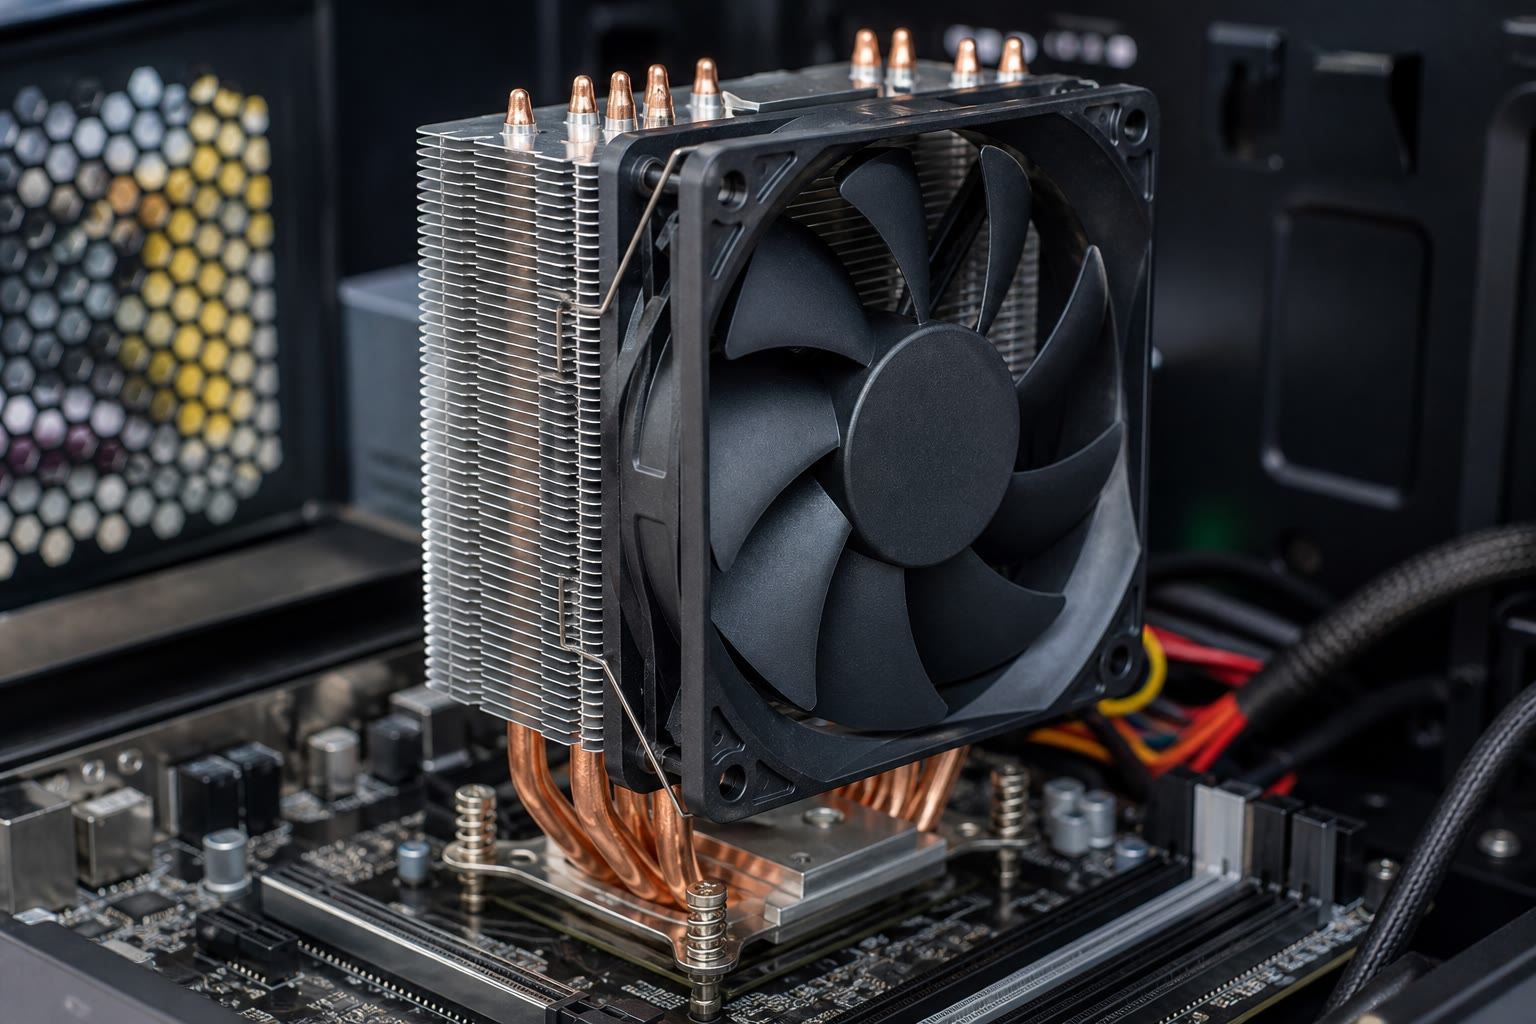
\includegraphics[width=0.58\linewidth]{images/book4/ai/b4-25-cpu-heat-sink.jpg}

{\small 处理器上的翅片式散热器：一百瓦热量从一平方厘米的硅中传导出来，
经金属底座扩散开来，
再由翅片交给空气，翅片使散热面积增至原来的三十倍。}
\end{omfigure}

\section{傅里叶定律}

\begin{definition}[热流密度]\label{def:b2:heat-conduction:flux}
\emph{热流密度}\index{热流密度}
$\vect{j}_Q$（单位为\unit{W/m^2}）是这样一个矢量：
由传导输运的能量，
经有向面元 $\dd\vect S$，在 $\dd t$ 内为 $\vect{j}_Q\cdot\dd\vect S\,\dd t$；
而通过某一曲面的\emph{热流量}\index{热流量}（功率，单位为瓦特）
设该曲面为 $S$，则 $\Phi = \iint_S\vect{j}_Q\cdot\dd\vect S$。
\end{definition}

\begin{theorem}[傅里叶定律]\label{thm:b2:heat-conduction:fourier}
在温度不均匀的静止介质中，
\[
\vect{j}_Q = -\lambda\,\vect{\operatorname{grad}}\,T ,
\]
其中\emph{热导率}\index{热导率}
$\lambda > 0$（单位为\unit{W/m/K}）依赖于材料，且较弱地依赖于
温度。热量沿温度下降的方向流动，即从高温流向低温——
这正是线性定律中内含的热力学第二定律。
\end{theorem}

\begin{proof}
本定律是唯象的，与菲克定律一样，其微观依据也相同：
分子（或金属中的自由电子，或晶格振动）
携带能量做无规行走，
并且能量更多地来自高温一侧。
\end{proof}

\begin{example}[热导率]\label{ex:b2:heat-conduction:values}
金属（电子既传递热量，也传导电流——
两者的\omterm{thm:b2:heat-conduction:fourier}{热导率}彼此对应）：铜 \qty{400}{W/m/K}，铝
\qty{240}{W/m/K}，钢 \qty{50}{W/m/K}。绝缘固体：混凝土
\qty{1.5}{W/m/K}，玻璃 \qty{1}{W/m/K}，砖 \qty{0.8}{W/m/K}，木材
\qty{0.15}{W/m/K}。液体：水 \qty{0.6}{W/m/K}。气体：空气
\qty{0.026}{W/m/K}——而最好的绝热材料（玻璃棉或泡沫，
\omterm{thm:b2:heat-conduction:fourier}{热导率}约 \qty{0.04}{W/m/K}），主要是静止的空气，被封闭其中，使其无法
发生对流。从铜到空气，相差四个数量级。
\end{example}

\section{能量平衡与热传导方程}

\begin{theorem}[局部能量平衡]\label{thm:b2:heat-conduction:balance}
在密度为 $\rho$、比热容为
$c$ 的固体（或静止流体）中，单位体积释放的功率为 $p$（焦耳热、
化学或核反应、吸收的辐射），
\[
\rho c\,\frac{\partial T}{\partial t} = -\operatorname{div}\vect{j}_Q + p ,
\qquad\text{一维情形}\quad
\rho c\,\frac{\partial T}{\partial t} = -\frac{\partial j_Q}{\partial x} + p .
\]
\end{theorem}

\begin{proof}
对 $x$ 与 $x + \dd x$ 之间的薄片应用热力学第一定律（截面为 $S$，
体积固定，故不做功）：其内能 $\rho c\,T\,S\,\dd x$
在 $\dd t$ 内由于接收的热量而改变，$[j_Q(x) - j_Q(x+\dd x)]S\,\dd t
= -\partial_x j_Q\,\dd x\,S\,\dd t$，再加上 $p\,S\,\dd x\,\dd t$。在三
维情形中，经闭合曲面进入固定体积的热量
为 $-\iint\vect{j}_Q\cdot\dd\vect S = -\iiint\operatorname{div}\vect{j}_Q\,\dd\tau$。
\end{proof}

\begin{theorem}[热传导方程]\label{thm:b2:heat-conduction:equation}
若 $\lambda$、$\rho$、$c$ 均为常数，
\[
\frac{\partial T}{\partial t} = a\,\Delta T + \frac{p}{\rho c},
\qquad a = \frac{\lambda}{\rho c} \quad\text{（即\emph{热扩散率}\index{热扩散率}，单位为\unit{m^2/s}）} .
\]
\omterm{thm:b2:particle-diffusion:equation}{扩散方程}的全部结论都成立：线性、
不可逆性、平滑作用，以及标度 $L \sim \sqrt{at}$、$t \sim
L^2/a$.
\end{theorem}

\begin{proof}
将傅里叶定律代入平衡式：$\rho c\,\partial_t T =
\lambda\Delta T + p$.
\end{proof}

\begin{example}[热扩散率与时间]\label{ex:b2:heat-conduction:times}
铜的 $a = \qty{1.1e-4}{m^2/s}$，空气 \qty{2e-5}{m^2/s}，混凝土和
砖 $\approx \qty{5e-7}{m^2/s}$，水 \qty{1.4e-7}{m^2/s}，木材
\qty{1e-7}{m^2/s}。热量穿过一厘米厚的铜只需一秒，一厘米厚的
砖需要三分钟，厚 \qty{20}{cm} 的墙需要一天
（这正是厚墙能够平抑昼夜循环的原因），
半厚为 \qty{1.5}{cm} 的牛排，十五分钟即可烹熟（烹饪
时间与厚度的平方成正比），以及一千米厚的岩石
需 $10^{12}\,\unit{s}$，约三万年——地球仍在
从形成时起持续冷却。
\end{example}

\section{稳态：热阻}

\begin{proposition}[平板的热阻]\label{prop:b2:heat-conduction:resistance}
在无源的稳态下，厚度为 $e$、
面积为 $S$、\omterm{thm:b2:heat-conduction:fourier}{热导率}为 $\lambda$ 的平板，位于温度 $T_1$ 与
$T_2$ 之间，温度分布为线性，并携带\omterm{def:b2:heat-conduction:flux}{热流量}
\[
\Phi = \frac{T_1 - T_2}{R_{\text{阈}}}, \qquad
R_{\text{阈}} = \frac{e}{\lambda S}\quad\text{（单位 \unit{K/W}）} :
\]
称其为\emph{热阻}\index{热阻}。温度
扮演电势的角色，\omterm{def:b2:heat-conduction:flux}{热流量}则扮演电流的角色：串联的热阻
（如墙的各层）相加，并联的热阻（如墙与
窗）则取倒数相加。对于圆柱壳（如管道的
保温层），内、外半径分别为 $r_1 < r_2$、长为 $\ell$，
$R_{\text{阈}} = \ln(r_2/r_1)/2\pi\lambda\ell$；对于球壳，
$(1/r_1 - 1/r_2)/4\pi\lambda$。
\end{proposition}

\begin{proof}
$\dd^2T/\dd x^2 = 0$：温度呈仿射分布，$j_Q = \lambda(T_1 - T_2)/e$
为均匀量，$\Phi = j_QS$。在圆柱几何中，$\Phi = -\lambda\,2\pi
r\ell\,\dd T/\dd r$ 对每个 $r$ 都相同（无积累），故
$T = A - (\Phi/2\pi\lambda\ell)\ln r$；在球几何中，$\Phi =
-4\pi r^2\lambda\,\dd T/\dd r$ 给出 $T = A + \Phi/4\pi\lambda r$。
\end{proof}

\begin{proposition}[与流体的交换：牛顿定律]\label{prop:b2:heat-conduction:newton}
温度为 $T_{\text{s}}$ 的固体表面与流体接触，流体温度为 $T_{\text{f}}$
（远离表面处），损失的\omterm{def:b2:heat-conduction:flux}{热流密度}为
\[
j_Q = h\,(T_{\text{s}} - T_{\text{f}}) ,
\]
其中\emph{传热系数}\index{传热系数}
 $h$（单位 \unit{W/m^2/K}）综合了通过
紧贴壁面的薄流体层的传导，以及不断更新该层的
对流：对于空气，$h \approx 5$--\qty{25}{W/m^2/K}，自然对流或
弱对流时；强制对流时为 $50$--\qty{500}{W/m^2/K}，
对于水为 $10^3$--$10^4$。此外，表面还附加一个\emph{膜热阻}，
$1/hS$，与壁面串联。
\end{proposition}

\begin{proof}
唯象地处理：不计算流体的运动，而将其概括在
$h$ 中（由测量得到，或由流体力学的关联式给出）。
\end{proof}

\begin{omfigure}
\begin{tikzpicture}[scale=0.9, >=stealth]
  % wall layers
  \fill[omExo!15] (0,0) rectangle (1.6,2.6);
  \fill[omDef!12] (1.6,0) rectangle (2.6,2.6);
  \fill[gray!15] (2.6,0) rectangle (2.8,2.6);
  \draw (0,0) rectangle (2.8,2.6);
  \draw (1.6,0) -- (1.6,2.6); \draw (2.6,0) -- (2.6,2.6);
  \node[font=\scriptsize] at (0.8,2.85) {砖};
  \node[font=\scriptsize] at (2.1,2.85) {玻璃棉};
  \node[font=\scriptsize, right] at (2.9,1.3) {室内 $T_{\text{i}}$};
  \node[font=\scriptsize, left] at (-0.1,1.3) {室外 $T_{\text{o}}$};
  \draw[->, omThm, thick] (3.6,0.7) -- (-0.8,0.7) node[midway, below, font=\scriptsize] {$\Phi$};
  % resistor chain
  \begin{scope}[yshift=-1.6cm]
    \draw (-0.8,0) -- (0.2,0);
    \draw (0.2,-0.18) rectangle (1.0,0.18); \node[font=\tiny] at (0.6,0) {$1/h_{\text{o}}S$};
    \draw (1.0,0) -- (1.4,0);
    \draw (1.4,-0.18) rectangle (2.4,0.18); \node[font=\tiny] at (1.9,0) {$e_1/\lambda_1 S$};
    \draw (2.4,0) -- (2.8,0);
    \draw (2.8,-0.18) rectangle (3.8,0.18); \node[font=\tiny] at (3.3,0) {$e_2/\lambda_2 S$};
    \draw (3.8,0) -- (4.2,0);
    \draw (4.2,-0.18) rectangle (5.0,0.18); \node[font=\tiny] at (4.6,0) {$1/h_{\text{i}}S$};
    \draw (5.0,0) -- (5.6,0);
    \fill (-0.8,0) circle (1.5pt) node[above, font=\scriptsize] {$T_{\text{o}}$};
    \fill (5.6,0) circle (1.5pt) node[above, font=\scriptsize] {$T_{\text{i}}$};
  \end{scope}
  % profile
  \begin{scope}[xshift=7.2cm]
    \draw[->] (0,0) -- (3.4,0) node[right, font=\scriptsize] {$x$};
    \draw[->] (0,0) -- (0,2.8) node[above, font=\scriptsize] {$T$};
    \draw[omDef, thick] (0,0.4) -- (0.3,0.6) -- (1.6,0.9) -- (2.6,2.4) -- (2.8,2.45) -- (3.2,2.6);
    \draw[dashed] (0.3,0) -- (0.3,0.6); \draw[dashed] (1.6,0) -- (1.6,0.9); \draw[dashed] (2.6,0) -- (2.6,2.4); \draw[dashed] (2.8,0) -- (2.8,2.45);
    \node[font=\scriptsize, below] at (0.95,0) {砖};
    \node[font=\scriptsize, below] at (2.1,0) {玻璃棉};
    \node[font=\scriptsize, left] at (0,0.4) {$T_{\text{o}}$};
    \node[font=\scriptsize, right] at (3.2,2.6) {$T_{\text{i}}$};
  \end{scope}
\end{tikzpicture}

{\small 复合墙及其热等效电路：膜、砖、玻璃棉、
膜依次串联。右图为温度分布——几乎全部温降
落在热阻最大的一层——玻璃棉上，
尽管它是最薄的一层。}
\end{omfigure}

\begin{example}[墙与窗]\label{ex:b2:heat-conduction:wall}
每平方米：砖厚 \qty{20}{cm}，\omterm{thm:b2:heat-conduction:fourier}{热导率}为 \qty{0.8}{W/m/K}，$R =
\qty{0.25}{m^2.K/W}$；两层膜，$1/8 + 1/25 = \qty{0.165}{m^2.K/W}$：
总热阻为 $0.415$，即 $U = 1/R = \qty{2.4}{W/m^2/K}$，温差为 \qty{20}{K} 时，
热流为 \qty{48}{W/m^2}。再加 \qty{10}{cm} 厚的玻璃棉，$R =
\qty{2.5}{m^2.K/W}$：总热阻为 $2.9$，$U = \qty{0.34}{W/m^2/K}$——
降为原来的七分之一。单层玻璃，厚 \qty{4}{mm}，\omterm{thm:b2:heat-conduction:fourier}{热导率}为 \qty{1}{W/m/K}，
几乎全是膜热阻：$R = 0.004 + 0.165$，$U \approx \qty{6}{W/m^2/K}$；
在两层玻璃之间夹一层 \qty{12}{mm} 的静止空气，增加热阻 $0.012/0.026 =
\qty{0.46}{m^2.K/W}$，使散热损失降为原来的三分之一以下。
\end{example}

\begin{definition}[毕渥数]\label{def:b2:heat-conduction:biot}
对于与流体进行热交换的尺度为 $L$ 的固体，
称\emph{毕渥数}\index{毕渥数}为
\[
\mathrm{Bi} = \frac{hL}{\lambda} = \frac{\text{内阻 } L/\lambda S}{\text{膜热阻 } 1/hS}
\]
它比较两者。若 $\mathrm{Bi} \ll 1$，固体在任一时刻温度都是均匀的，
整体一起降温，按指数规律
以时间常数 $\tau = \rho c V/hS$ 变化；若 $\mathrm{Bi} \gg 1$，则
表面温度与流体相同，内部则以自身的节奏导热，
其特征时间为 $L^2/a$。
\end{definition}

\section{周期性加热：热波}

\begin{proposition}[半空间中的热波]\label{prop:b2:heat-conduction:wave}
若半空间的表面 $x = 0$ 保持 $T(0,t) = T_0 +
\theta_0\cos\omega t$，则内部温度
在稳定阶段为
\[
T(x,t) = T_0 + \theta_0\,\eu^{-x/\delta}\cos\Big(\omega t - \frac{x}{\delta}\Big),
\qquad \delta = \sqrt{\frac{2a}{\omega}} :
\]
这是一列向内传播的波，速率为 $\omega\delta =
\sqrt{2a\omega}$，每弧度相位衰减一个\emph{穿透深度} $\delta$
——即每个波长衰减 $\eu^{-2\pi} = 2 \times 10^{-3}$
倍。快振荡比慢振荡穿透得更浅。
\end{proposition}

\begin{proof}
试取 $\underline T = \theta_0\eu^{\iu(\omega t - \underline k x)}$：
由 $\iu\omega = -a\underline k^2$ 得 $\underline k^2 = -\iu\omega/a$，
于是 $\underline k = (1 - \iu)\sqrt{\omega/2a} = (1 - \iu)/\delta$（取
在 $x > 0$ 时衰减的根）。取实部即可。
\end{proof}

\begin{omfigure}
\begin{tikzpicture}
  \begin{axis}[omaxis, width=9cm, height=4.8cm, xmin=0, xmax=4.6, ymin=-1.1, ymax=1.1,
    xlabel={$x/\delta$}, ylabel={$(T - T_0)/\theta_0$}, xtick={1,2,3,4}, ytick={-1,1}, clip=false,
    axis x line=middle, axis y line=left,
    legend style={font=\scriptsize, at={(0.98,0.04)}, anchor=south east, draw=none, fill=none}]
    \addplot[omDef, thick, domain=0:4.6, samples=120] {exp(-x)*cos(deg(-x))};
    \addlegendentry{$\omega t = 0$}
    \addplot[omThm, thick, domain=0:4.6, samples=120] {exp(-x)*cos(deg(pi/2-x))};
    \addlegendentry{$\omega t = \pi/2$}
    \addplot[omExo, thick, domain=0:4.6, samples=120] {exp(-x)*cos(deg(pi-x))};
    \addlegendentry{$\omega t = \pi$}
    \addplot[gray, dashed, domain=0:4.6, samples=60] {exp(-x)};
    \addplot[gray, dashed, domain=0:4.6, samples=60] {-exp(-x)};
  \end{axis}
\end{tikzpicture}

{\small 三个时刻的热波：表面的振荡
以阻尼波的形式穿透，其振幅按 $\eu^{-x/\delta}$
衰减（虚线），相位滞后 $x/\delta$——在 $x = \pi\delta$ 处
温度与表面温度相反。}
\end{omfigure}

\begin{example}[土壤、地窖与葡萄酒]\label{ex:b2:heat-conduction:soil}
土壤的 $a \approx \qty{5e-7}{m^2/s}$。日周期，$\omega = 2\pi/\qty{86400}{s}$：
$\delta = \qty{12}{cm}$——地下半米处，日间变化便已消失。年周期：
$\delta = \qty{2.2}{m}$；在该深度，\qty{10}{K} 的夏–冬温差
降至 \qty{3.7}{K}，且滞后一弧度，即两个月：地窖
在三月最冷，九月最暖；在 \qty{5}{m} 深处，
温度与恒定值仅相差 \qty{1}{K}——这正是能储存葡萄酒的地窖。
同样的数学也给出电磁学中的\omterm{def:b2:dispersion-wave-packets:complex}{趋肤深度}
（\cref{ch:b2:waves-in-media}）：方程相同，都是 $\sqrt{2/(\text{热扩散率}
\times\omega)}$。
\end{example}

\section{翅片}

\begin{proposition}[冷却翅片]\label{prop:b2:heat-conduction:fin}
细棒或薄板（截面 $S$，周长 $p$，\omterm{thm:b2:heat-conduction:fourier}{热导率} $\lambda$）
在 $x = 0$ 处与温度为 $T_0$ 的壁面相连，置于温度为 $T_{\text{f}}$ 的流体中，
表面\omterm{prop:b2:heat-conduction:newton}{传热系数}为 $h$，其过余温度 $\theta = T - T_{\text{f}}$
满足
\[
\frac{\dd^2\theta}{\dd x^2} = m^2\theta, \qquad m = \sqrt{\frac{hp}{\lambda S}} ;
\]
对于长翅片，$\theta = \theta_0\eu^{-mx}$，翅片散出的热流为 $\Phi =
\sqrt{hp\lambda S}\,\theta_0$——相当于一段长为 $\sqrt{\lambda
S/hp} = 1/m$ 的裸露表面散出的热流，温度降至 $\theta_0/\eu$ 时位于 $x = 1/m$ 处。
对于有限长 $L$ 的翅片（末端绝热），$\theta =
\theta_0\cosh m(L-x)/\cosh mL$，其\emph{效率}\index{翅片效率}
——即其热流与温度为 $\theta_0$ 的等温翅片热流之比——
为 $\eta = \tanh(mL)/mL$。
\end{proposition}

\begin{proof}
对微元段 $[x, x + \dd x]$ 作稳态平衡：传入热流
$-\lambda S\theta'(x)$；传出的热流 $-\lambda S\theta'(x + \dd x)$；
流体带走的热量 $hp\,\theta\,\dd x$：$\lambda S\theta'' = hp\theta$。翅片根部的热流
为 $-\lambda S\theta'(0)$：长翅片为 $\lambda Sm\theta_0$，
有限长翅片为 $\lambda Sm\theta_0\tanh mL$，应与
$hpL\theta_0$ 比较。翅片厚度方向的\omterm{def:b2:heat-conduction:biot}{毕渥数} $ht/\lambda$ 必须
很小，方可进行一维处理。
\end{proof}

\begin{omfigure}
\begin{tikzpicture}
  \begin{axis}[omaxis, width=6.4cm, height=4.4cm, xmin=0, xmax=3.2, ymin=0, ymax=1.12,
    xlabel={$mx$}, ylabel={$\theta/\theta_0$}, xtick={1,2,3}, ytick={1}, clip=false,
    legend style={font=\scriptsize, at={(0.98,0.98)}, anchor=north east, draw=none, fill=none}]
    \addplot[omDef, thick, domain=0:3.2, samples=60] {exp(-x)};
    \addlegendentry{长翅片}
    \addplot[omExo, thick, domain=0:1.2, samples=60] {cosh(1.2-x)/cosh(1.2)};
    \addlegendentry{$mL = 1.2$}
    \addplot[omThm, thick, domain=0:0.5, samples=30] {cosh(0.5-x)/cosh(0.5)};
    \addlegendentry{$mL = 0.5$}
  \end{axis}
  \begin{scope}[xshift=7.2cm, yshift=0.3cm, scale=0.8, >=stealth]
    \fill[gray!25] (0,0) rectangle (0.5,3.2);
    \fill[omDef!20] (0.5,1.4) rectangle (4.2,1.8);
    \draw (0.5,1.4) rectangle (4.2,1.8);
    \node[font=\scriptsize, rotate=90] at (0.25,1.6) {壁面 $T_0$};
    \draw[->, omThm, thick] (0.6,1.6) -- (1.6,1.6) node[right, font=\scriptsize] {$-\lambda S\theta'$};
    \foreach \x in {1.2,2.0,2.8,3.6}{
      \draw[->, omExo] (\x,1.85) -- (\x,2.4);
      \draw[->, omExo] (\x,1.35) -- (\x,0.8);
    }
    \node[font=\scriptsize, omExo] at (2.4,2.7) {$hp\,\theta\,\dd x$};
    \node[font=\scriptsize] at (2.4,0.45) {流体 $T_{\text{f}}$};
  \end{scope}
\end{tikzpicture}

{\small 左：沿翅片的温度分布，给出长翅片及两个有限长翅片
（绝热端）的情形——超过 $mx \approx 2$ 后，翅片增益很小。右：
一薄片的热平衡：沿片方向的传导，以及经周界向外的
对流。}
\end{omfigure}

\begin{example}[散热器]\label{ex:b2:heat-conduction:sink}
铝制翅片厚 \qty{1}{mm}（$p/S \approx 2/t = \qty{2000}{m^{-1}}$），
\qty{30}{mm} 高，置于强制对流空气中，$h = \qty{50}{W/m^2/K}$：$m =
\sqrt{2h/\lambda t} = \qty{20}{m^{-1}}$，$mL = 0.6$，$\eta = 0.89$——翅片以其
面积的 $89\%$ 发挥作用。共三十片，宽 \qty{60}{mm}，
可提供 \qty{0.11}{m^2} 的散热面积，而裸露的 \qty{60}{mm} 见方底面
仅提供 \qty{0.0036}{m^2}。热阻为 $1/\eta hA = \qty{0.2}{K/W}$，而非
\qty{5.6}{K/W}；\qty{100}{W} 的热流使底座升温 \qty{20}{K}，而非
\qty{560}{K}。加长翅片增益甚小（$\tanh$ 趋于饱和），更薄的翅片则
效率下降：$mL \approx 1$ 是工程上的折中。
\end{example}

\section{传导产生的熵}

\begin{proposition}[熵的产生]\label{prop:b2:heat-conduction:entropy}
热流 $\Phi$ 从温度为 $T_{\text{h}}$ 的物体传导至温度为
$T_{\text{c}} < T_{\text{h}}$ 的物体，经一稳定壁面时，以
下述速率产生熵：
\[
\dot S_{\text{c}} = \Phi\Big(\frac{1}{T_{\text{c}}} - \frac{1}{T_{\text{h}}}\Big) > 0 ;
\]
局域地，传导每单位体积、单位时间产生 $\sigma_s = \lambda\,(\vect{\operatorname{grad}}\,T)^2/T^2
\ge 0$——仅在温度
处处均匀处为零。热传导不可逆：同样的能量，以
较低温度传递，所能做的功更少。
\end{proposition}

\begin{proof}
壁面状态不变，其熵为常量：热体
每单位时间失去 $\Phi/T_{\text{h}}$，冷体
获得 $\Phi/T_{\text{c}}$；两者之差即为所产生的熵。局域地，熵
平衡式为 $\partial_t(\rho s) + \operatorname{div}(\vect{j}_Q/T) = \sigma_s$
由 $\rho T\partial_t s = -\operatorname{div}\vect{j}_Q$ 得 $\sigma_s =
\vect{j}_Q\cdot\vect{\operatorname{grad}}(1/T) = -\vect{j}_Q\cdot
\vect{\operatorname{grad}}\,T/T^2 = \lambda(\vect{\operatorname{grad}}\,T)^2/T^2$.
\end{proof}

\begin{method}[传导估算]\label{meth:b2:heat-conduction:method}
(1) 稳态：画出热阻网络——平板 $e/\lambda S$，表面膜 $1/hS$，
圆筒壳 $\ln(r_2/r_1)/2\pi\lambda\ell$；串联与并联。
(2) 暂态：$\mathrm{Bi} = hL/\lambda$；若较小，则 $\tau = \rho cV/hS$；若
较大，则 $t \sim L^2/a$。(3) 周期性：$\delta = \sqrt{2a/\omega}$，阻尼
$\eu^{-x/\delta}$，滞后 $x/\delta$。(4) 源项：每单位体积 $p$，抛物
线形分布。(5) 翅片：$m = \sqrt{hp/\lambda S}$，$\eta = \tanh(mL)/mL$。(6)
熵：$\Phi(1/T_{\text{c}} - 1/T_{\text{h}})$。
\end{method}

\section{练习}

\begin{exercise}[$\star$]\label{exo:b2:heat-conduction:1}
一堵厚 \qty{20}{cm} 的砖墙（$\lambda = \qty{0.8}{W/m/K}$），面积 \qty{100}{m^2}，
置于室内 \qty{20}{\celsius} 与室外 \qty{0}{\celsius} 之间
（表面温度即为上述温度）：求\omterm{def:b2:heat-conduction:flux}{热流密度}与总热流；再求
加装 \qty{10}{cm} 玻璃棉（\qty{0.04}{W/m/K}）后的结果。
\end{exercise}

\begin{exercise}[$\star$]\label{exo:b2:heat-conduction:2}
计算下列材料的\omterm{thm:b2:heat-conduction:equation}{热扩散率}：铜（$\lambda = 400$，$\rho = 8900$，$c = \qty{385}{J/kg/K}$），
混凝土（$1.5$，$2300$，$900$），木材（$0.15$，$600$，$2500$）。求热量穿过
每种材料 \qty{1}{cm} 与 \qty{20}{cm} 厚度所需的时间，以及
地球 \qty{30}{km} 厚地壳的情形。
\end{exercise}

\begin{exercise}[$\star$]\label{exo:b2:heat-conduction:3}
单层玻璃（\qty{4}{mm}，$\lambda = \qty{1}{W/m/K}$），表面膜 $h_{\text{i}}
= 8$，$h_{\text{o}} = \qty{25}{W/m^2/K}$；双层玻璃，中间夹 \qty{12}{mm}
厚的静止空气层（\qty{0.026}{W/m/K}）：求 $U$ 值及
\qty{20}{K} 温差下的热流。实际双层玻璃的散热约为
此估算值的两倍？氩气与低发射率镀膜各起何作用？
\end{exercise}

\begin{exercise}[$\star$]\label{exo:b2:heat-conduction:4}
烹饪：肉类的\omterm{thm:b2:heat-conduction:equation}{热扩散率} $a = \qty{1.4e-7}{m^2/s}$。求
厚 \qty{3}{cm} 牛排中心感受到锅温所需的时间；厚 \qty{12}{cm} 烤肉的情形。若火鸡
的质量加倍，需多花多少时间（线度与质量的
立方根成正比）？
\end{exercise}

\begin{exercise}[$\star\star$]\label{exo:b2:heat-conduction:5}
\emph{内部热源。}半径为 $R$ 的圆柱体，单位体积释放 $p$
的热量；表面温度为 $T_{\text{s}}$。(a) 证明：$T(r) = T_{\text{s}} +
p(R^2 - r^2)/4\lambda$。(b) 铜线，$R = \qty{1}{mm}$，$j =
\qty{1e7}{A/m^2}$，$\gamma = \qty{6e7}{S/m}$：求 $p$ 及中心与表面
温差。(c) 核燃料棒，$R = \qty{5}{mm}$，$p = \qty{3e8}{W/m^3}$，
$\lambda = \qty{3}{W/m/K}$：求同样的问题。(d) 对结果加以讨论。
\end{exercise}

\begin{exercise}[$\star\star$]\label{exo:b2:heat-conduction:6}
\emph{地下温度。}(a) 推导 $\delta = \sqrt{2a/\omega}$。(b) 土壤，
$a = \qty{5e-7}{m^2/s}$：求日变与年变的穿透深度。(c) 求
使年振幅为地表年振幅十分之一的
深度，以及该处的相位滞后。(d) 水管在冬季表面
温度降至 \qty{-10}{\celsius}，平均值为
\qty{10}{\celsius} 时，不得冻结：求最小埋深（年波）。
\end{exercise}

\begin{exercise}[$\star\star$]\label{exo:b2:heat-conduction:7}
\emph{\omterm{def:b2:heat-conduction:biot}{毕渥数}。}(a) 铜球，半径 \qty{1}{cm}，置于空气中（$h =
\qty{10}{W/m^2/K}$）：求\omterm{def:b2:heat-conduction:biot}{毕渥数}及其冷却的时间常数。(b) 一
个土豆（$\lambda = \qty{0.5}{W/m/K}$，$a = \qty{1.4e-7}{m^2/s}$，半径
\qty{3}{cm}）置于 $h = \qty{20}{W/m^2/K}$ 的烤箱中：求\omterm{def:b2:heat-conduction:biot}{毕渥数}，并判断
哪种时间支配其烹饪？(c) 热电偶的热结点为何做得很小？
(d) 一杯咖啡在搅拌或吹气时为何冷却得更快——
改变的是哪一项热阻？
\end{exercise}

\begin{exercise}[$\star\star$]\label{exo:b2:heat-conduction:8}
\emph{肋片。}(a) 推导 $\theta'' = m^2\theta$，并求长肋片的解。
(b) 铝制肋片，厚 \qty{1}{mm}，高 \qty{30}{mm}，自然
对流 $h = \qty{20}{W/m^2/K}$：求 $m$、$mL$ 及效率。(c) 肋片
使其底面换热面积增大为原来的多少倍，以及
热流增大为原来的多少倍？(d) 为何过长或过细的肋片是金属的浪费？
\end{exercise}

\begin{exercise}[$\star\star$]\label{exo:b2:heat-conduction:9}
\emph{管道。}(a) 推导圆柱壳层的热阻。(b) 一根蒸汽管，
外半径 \qty{5}{cm}，温度为 \qty{150}{\celsius}，外包
\qty{5}{cm} 厚的玻璃棉，外侧空气温度 \qty{20}{\celsius}，外侧\omterm{prop:b2:heat-conduction:newton}{传热系数} $h =
\qty{10}{W/m^2/K}$：求每米长的热损失，并与裸管比较。
(c) 证明保温层与膜层的总热阻在
\emph{临界半径} $r_{\text{c}} = \lambda/h$ 处取最小值。(d) 对于一根
半径为 \qty{1}{mm} 的电线，外包塑料护套（$\lambda =
\qty{0.2}{W/m/K}$），护套使铜降温还是升温？
\end{exercise}

\begin{exercise}[$\star\star\star$]\label{exo:b2:heat-conduction:10}
\emph{熵。}\cref{exo:b2:heat-conduction:1}中的墙壁（未加保温），
两侧温度分别为 \qty{293}{K} 与 \qty{273}{K}。(a) 每秒产生的熵。
(b) 利用线性分布计算 $\int\sigma_s\,\dd V$，并检验其
结果一致。(c) 加保温后产生的熵。(d) 可逆热机在这两温度之间
能从这两温度间传递的 \qty{8}{kW} 中提取的功，
以及穿过墙壁后尚余多少。
\end{exercise}

\begin{exercise}[$\star\star\star$]\label{exo:b2:heat-conduction:11}
\emph{金属为何摸起来冷。}(a) 对于热波，计算
表面热流 $j_Q(0,t)$，并证明它比表面温度超前
$\pi/4$，振幅为 $\sqrt{\lambda\rho c\,\omega}\,\theta_0$。其中
$b = \sqrt{\lambda\rho c}$ 称为\emph{热渗透系数}。(b) 两个
半无限大物体分别处于 $T_1$ 与 $T_2$，并使其接触。在本阶段不加证明地承认：
接触后两者各自服从 erfc 型分布，且具有共同的
表面温度 $T_{\text{c}}$，并写出接触面处热流连续的条件，
证明 $T_{\text{c}} = (b_1T_1 + b_2T_2)/(b_1 + b_2)$。(c) 皮肤
（$b \approx \qty{1000}{J/m^2/K/s^{1/2}}$，\qty{33}{\celsius}）分别
与 \qty{20}{\celsius} 的铜（$b = 37000$）或木材（$b = 400$）接触时，求接触温度。
(d) 为何在相同温度下，瓷砖地面摸起来比地毯更冷，
而这种感觉为何只是暂态的？
\end{exercise}

\begin{exercise}[$\star\star\star$]\label{exo:b2:heat-conduction:12}
\emph{平板冷却。}位于 $-L < x < L$ 内的平板，初温为 $T_0$，于 $t =
0$ 时被投入温度为 $T_{\text{f}}$ 的浴槽中（$h \to \infty$）。(a) 证明 $\theta =
T - T_{\text{f}}$ 有形如 $\cos(k_nx)\,\eu^{-ak_n^2t}$ 的解，其中 $k_n
= (2n+1)\pi/2L$。(b) 将初始条件按这些模式展开为
傅里叶级数，并写出完整解。(c) 经过最初的一段时间后，
哪一模式留存？其时间常数是多少？(d) 求
\qty{3}{cm} 牛排（$a = \qty{1.4e-7}{m^2/s}$）中心温度
与浴槽温度之差在 $1\%$ 以内所需的时间。
\end{exercise}

\section{问题：房屋保温与处理器冷却}

\begin{problem}[{周末问题——建筑尺度与芯片尺度上的
热传导}]\label{pb:b2:heat-conduction:1}
已知：砖 $\lambda = \qty{0.8}{W/m/K}$，$\rho = \qty{1800}{kg/m^3}$，$c =
\qty{840}{J/kg/K}$；玻璃棉 \qty{0.04}{W/m/K}；玻璃 \qty{1}{W/m/K}；静止
空气 \qty{0.026}{W/m/K}；铝 \qty{240}{W/m/K}，$\rho = \qty{2700}{kg/m^3}$，
$c = \qty{900}{J/kg/K}$；硅 \qty{150}{W/m/K}；导热硅脂
\qty{5}{W/m/K}；土壤 $a = \qty{5e-7}{m^2/s}$，$\lambda = \qty{1}{W/m/K}$；
膜层 $h_{\text{i}} = 8$，$h_{\text{o}} = \qty{25}{W/m^2/K}$。

\textbf{第一部分——房屋。}
房屋有 \qty{100}{m^2} 的墙壁（砖墙厚 \qty{20}{cm}）和 \qty{20}{m^2}
的单层玻璃窗（厚 \qty{4}{mm}）；室内 \qty{20}{\celsius}，
室外 \qty{0}{\celsius}。
\begin{enumerate}
  \item 仅砖墙的单位面积热阻；若其两侧分别
        处于两个温度，求\omterm{def:b2:heat-conduction:flux}{热流密度}。
  \item 计入两侧膜层后，每平方米的 $R$ 与 $U = 1/R$；加入
        \qty{10}{cm} 玻璃棉后，求同样的量。
  \item 单层玻璃窗的 $U$；双层玻璃窗
        中间夹 \qty{12}{mm} 静止空气层时的值。
  \item 墙壁加保温与窗户改为双层之前和之后，房屋的
        总热损失。
  \item 供暖季 $2500$ 度日（即温差在该季内的积分，
        单位 \unit{K.day}），求改造前后所损失的能量，
        以千瓦时计。
  \item 墙壁内表面温度（未保温与保温两种情形）；
        寒冷的墙面为何令人不适，并易滋生霉菌？
  \item 热量穿过砖墙的扩散时间；它对
        昼夜循环有何影响？
\end{enumerate}

\textbf{第二部分——房屋下方的土壤。}
\begin{enumerate}[resume]
  \item 推导热波的穿透深度
        $\delta = \sqrt{2a/\omega}$。
  \item 求土壤中日周期与年周期的 $\delta$。
  \item 求日振幅降至 $1\%$ 时的深度；求
        地表振幅为 \qty{10}{K} 时，\qty{2.2}{m} 与 \qty{5}{m} 深处
        的年振幅。
  \item 在 \qty{2.2}{m} 深处的相位滞后，以天计；地窖何时最冷？
  \item 求年周期热波的表面热流（包括振幅与相位）；
        将其振幅与地热流 \qty{0.06}{W/m^2} 作比较。
  \item 地热\omterm{def:b2:maxwell-equations:operators}{梯度}为 \qty{30}{K/km}，请据地热流与 $\lambda$ 检验其
        是否合理，并解释它为何在地窖的
        季节变化中不可见。
\end{enumerate}

\textbf{第三部分——处理器。}
芯片耗散功率 \qty{100}{W}，管芯面积 \qty{1}{cm^2}，厚 \qty{0.5}{mm}；
\qty{50}{\micro m} 厚的导热硅脂层覆盖 \qty{10}{cm^2} 的面积，将其粘接到
铝制散热器：底座 \qty{60}{mm} $\times$ \qty{60}{mm} $\times$
\qty{5}{mm}，三十片翅片，宽 \qty{60}{mm}，高 \qty{30}{mm}，厚 \qty{1}{mm}，
风扇给出 $h = \qty{50}{W/m^2/K}$；环境温度 \qty{25}{\celsius}。
\begin{enumerate}[resume]
  \item 穿过管芯的\omterm{def:b2:heat-conduction:flux}{热流密度}；管芯的热阻。
  \item 导热硅脂的热阻；若以 \qty{50}{\micro m} 的空气间隙
        替代它，热阻又为多少。
  \item 求翅片参数 $m$、$mL$ 及效率；检验
        沿翅片厚度方向的\omterm{def:b2:heat-conduction:biot}{毕渥数}。
  \item 翅片总面积与翅片的热阻；基底的
        热阻（经 \qty{5}{mm} 的传导）；结温。
  \item 若不加翅片（裸露的 \qty{60}{mm} 见方底座），重新计算并作结论。
  \item 风扇停转（$h = \qty{10}{W/m^2/K}$）：求结温；
        处理器在 \qty{100}{\celsius} 时会怎样？
  \item 求散热器的质量与热容；其时间常数 $RC$；
        以及单独管芯（\qty{0.1}{g}，\qty{700}{J/kg/K}）的时间常数。
  \item 优质散热器为何采用铜底座或热管？
\end{enumerate}

\textbf{第四部分——熵。}
\begin{enumerate}[resume]
  \item 未加保温的房屋围护结构每秒产生的熵
        （第 4 问）在 \qty{293}{K} 与 \qty{273}{K} 之间；
        以及保温后的情形。
  \item 芯片耗散的 \qty{100}{W} 由结传至环境时产生的熵；
        以及管芯中电功转化为热时
        产生的熵。
  \item 证明对平板有 $\int\sigma_s\,\dd V = \Phi(1/T_{\text{c}} -
        1/T_{\text{h}})$。
  \item 用五行概括墙壁、翅片、地窖
        与芯片各由什么支配。
\end{enumerate}
\end{problem}
